\section{Phân tích Dữ liệu và Trực quan hóa}
\label{sec:visualization}

Chương này trình bày chi tiết các biểu đồ phân tích và diễn giải kết quả cho bốn mục tiêu đã xác định ở Chương~\ref{sec:analysis_goals}. Các biểu đồ được thiết kế trực quan bằng Vega-Lite/Deneb kết hợp với các bộ lọc tương tác để làm nổi bật những phát hiện quan trọng nhất.

\subsection{Tổng quan và xu hướng thời gian}

\textbf{Mục tiêu}: Phân tích sự biến động của tổng số vụ va chạm trong giai đoạn 2020--2024, đồng thời xác định các khung thời gian có tần suất tai nạn cao bất thường.

\textbf{Biểu đồ thực tế}:
\begin{itemize}
    \item Biểu đồ cột xếp chồng (Stacked Bar Chart): Thể hiện tổng số vụ va chạm theo từng năm, phân loại theo khu vực Thành thị/Nông thôn.
    \item Biểu đồ bản đồ nhiệt (Heatmap Matrix): Thể hiện mật độ số vụ va chạm theo từng thứ trong tuần và khung giờ trong ngày (00:00 -- 23:00).
    \item Biểu đồ cột (Bar Chart): Thể hiện biến động tổng số vụ va chạm theo từng tháng trong năm.
    \item Biểu đồ đường (Line Chart): Thể hiện xu hướng tai nạn phân theo mức độ nghiêm trọng (Tử vong, Nghiêm trọng, Nhẹ) qua các năm 2020--2024.
\end{itemize}

\textbf{Nhận xét rút ra từ dữ liệu}:
\begin{itemize}
    \item \textbf{Xu hướng theo năm và khu vực}: Tổng số vụ va chạm tăng mạnh từ 2020 và đạt đỉnh vào 2022, sau đó có dấu hiệu giảm nhẹ về năm 2024. Đáng chú ý, các vụ tai nạn diễn ra ở khu vực Thành thị (màu xanh sáng) luôn chiếm tỷ trọng lớn hơn hẳn so với khu vực Nông thôn.
    \item \textbf{Mật độ va chạm theo Thứ và Giờ}: Tai nạn tập trung dày đặc vào các ngày làm việc trong tuần (Thứ 2 đến Thứ 6). Đỉnh điểm rủi ro rơi vào khung giờ tan tầm buổi chiều từ 15h00 đến 18h00 (đậm nhất ở dải 16h00 -- 17h00), tương đồng với thời gian lưu lượng giao thông đông đúc. Vào cuối tuần, mật độ tai nạn giảm đi rõ rệt.
    \item \textbf{Biến động theo tháng}: Tần suất va chạm có dấu hiệu tăng cao hơn vào những tháng cuối năm (từ Tháng 9 đến Tháng 11). Tháng 10 thường là tháng ghi nhận số lượng tai nạn cao nhất, có thể liên quan đến điều kiện thời tiết bắt đầu chuyển mùa.
    \item \textbf{Mức độ nghiêm trọng khá ổn định}: Mặc dù tổng số vụ va chạm biến động qua các năm, tỷ trọng các vụ ở mức độ Nhẹ vẫn chiếm áp đảo tuyệt đối. Đường xu hướng của các vụ án Tử vong (màu đỏ) và Nghiêm trọng (màu vàng) duy trì khá phẳng và ổn định, cho thấy mức độ thảm khốc không tăng đột biến so với mức tăng của tổng số vụ tai nạn chung.
\end{itemize}

\begin{figure}[H]
    \centering
    \begin{subfigure}{0.48\textwidth}
        \centering
        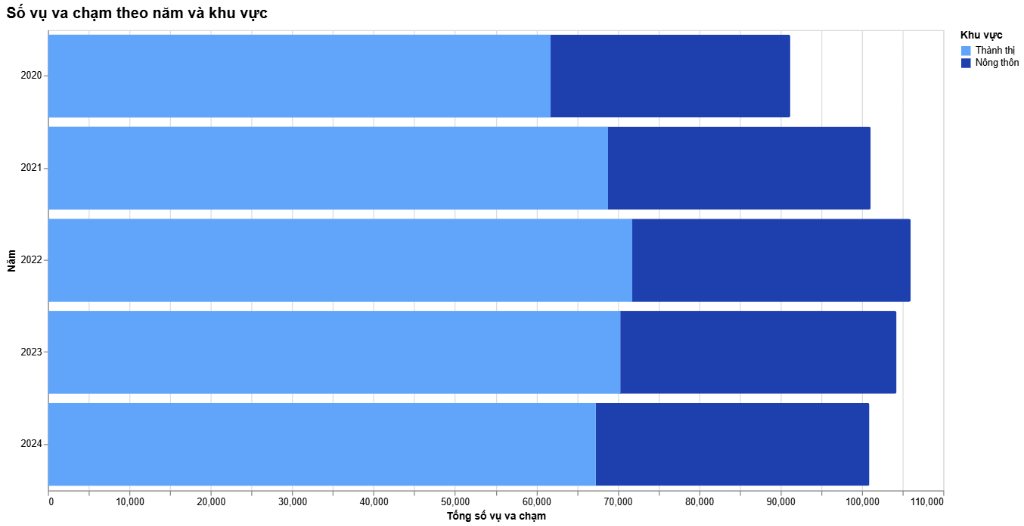
\includegraphics[width=\textwidth, keepaspectratio]{images/memberA_year_area.png}
        \caption{Số vụ theo năm và khu vực}
    \end{subfigure}
    \hfill
    \begin{subfigure}{0.48\textwidth}
        \centering
        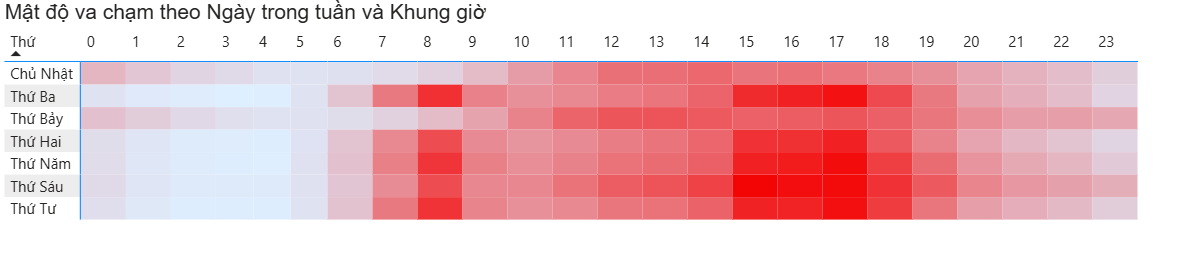
\includegraphics[width=\textwidth, keepaspectratio]{images/memberA_heatmap.png}
        \caption{Mật độ va chạm theo Thứ và Giờ}
    \end{subfigure}

    \vspace{0.3cm}

    \begin{subfigure}{0.48\textwidth}
        \centering
        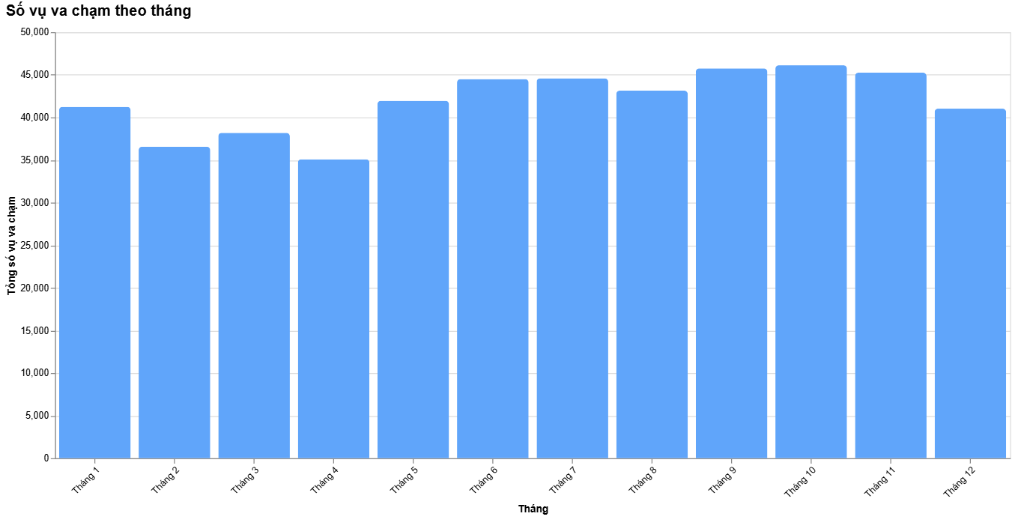
\includegraphics[width=\textwidth, keepaspectratio]{images/memberA_month.png}
        \caption{Số vụ va chạm theo tháng}
    \end{subfigure}
    \hfill
    \begin{subfigure}{0.48\textwidth}
        \centering
        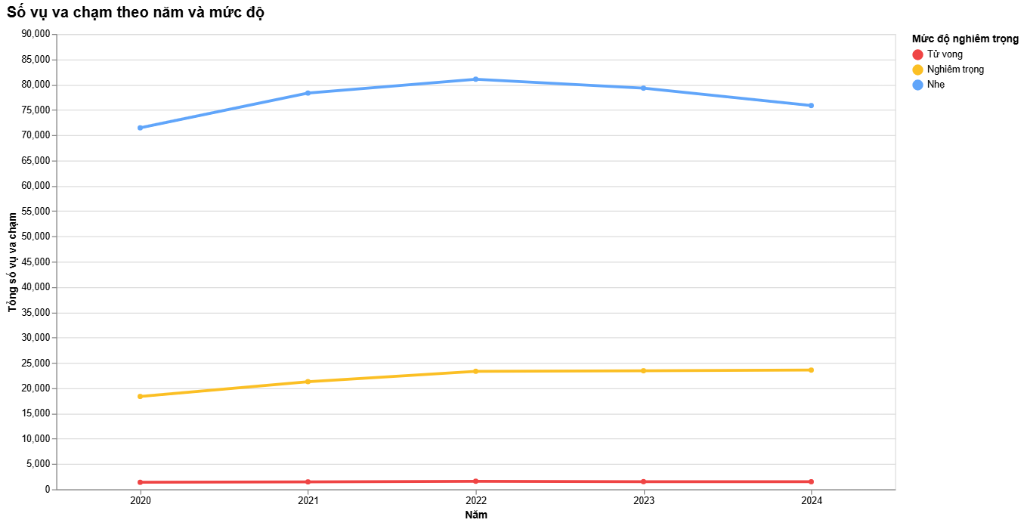
\includegraphics[width=\textwidth, keepaspectratio]{images/memberA_year_severity.png}
        \caption{Số vụ theo năm và mức độ}
    \end{subfigure}
    \caption{Các biểu đồ phân tích Tổng quan và xu hướng thời gian}
    \label{fig:memberA_charts}
\end{figure}

\subsection{Điều kiện đường sá và môi trường}


\textbf{Mục tiêu}: Phân tích sự ảnh hưởng của các điều kiện môi trường (thời tiết, ánh sáng) và đặc điểm hạ tầng (tình trạng mặt đường, loại đường, giới hạn tốc độ) đối với số lượng và mức độ nghiêm trọng của các vụ va chạm.

\textbf{Biểu đồ thực tế}:
\begin{itemize}
    \item Biểu đồ cột nhóm (Grouped Bar Chart): Thể hiện tổng số vụ va chạm theo tình trạng mặt đường, phân tách theo khu vực (Thành thị/Nông thôn).
    \item Biểu đồ bản đồ nhiệt (Heatmap Matrix): Thể hiện số vụ va chạm theo sự kết hợp giữa các điều kiện thời tiết và ánh sáng.
    \item Biểu đồ cột (Bar Chart): So sánh số lượng các vụ tai nạn diễn ra trên các tuyến đường có mức giới hạn tốc độ khác nhau.
    \item Biểu đồ cột xếp chồng (Stacked Bar Chart): Thể hiện số vụ va chạm phân bổ theo loại đường, phân lớp theo mức độ nghiêm trọng.
\end{itemize}

\textbf{Nhận xét rút ra từ dữ liệu}:
\begin{itemize}
    \item \textbf{Tình trạng mặt đường và Khu vực}: Hầu hết các vụ va chạm xảy ra trong điều kiện mặt đường "Khô ráo" ở khu vực "Thành thị" (khoảng 250 nghìn vụ). Mặc dù vậy, nhóm điều kiện "Ẩm ướt" vẫn ghi nhận một số lượng đáng kể tai nạn, cho thấy mặt đường trơn trượt vẫn là một rủi ro lớn. Ở hầu hết các tình trạng mặt đường, tai nạn tại khu vực Thành thị luôn chiếm ưu thế so với Nông thôn.
    \item \textbf{Thời tiết và Ánh sáng}: Tổ hợp có số vụ tai nạn cao nhất (thể hiện bằng ô màu xanh đậm nhất) là "Nắng (không gió)" kết hợp với "Ban ngày" với gần 300 nghìn vụ. Điều này hợp lý bởi đây là thời điểm lưu lượng xe cộ lưu thông đông nhất. Tổ hợp rủi ro lớn thứ hai là "Nắng (không gió)" đi kèm với "Tối (có đèn)". Các điều kiện thời tiết khắc nghiệt (Mưa, Tuyết, Sương mù) có số vụ va chạm tuyệt đối thấp hơn do người dân hạn chế ra đường.
    \item \textbf{Giới hạn tốc độ}: Đường có giới hạn tốc độ 30 mph (đặc trưng cho đường nội đô) ghi nhận số lượng tai nạn kỷ lục, vượt mốc 260 nghìn vụ. Đứng thứ hai là các cung đường giới hạn 20 mph (khoảng 80 nghìn vụ), và thứ ba là đường quốc lộ/ngoại ô giới hạn 60 mph. Điều này phản ánh thực tế rằng tai nạn dễ xảy ra hơn trong môi trường giao thông chằng chịt ở nội thành, dù tốc độ di chuyển không quá lớn.
    \item \textbf{Loại đường và mức độ nghiêm trọng}: Đường đơn (Single carriageway) chứng kiến số lượng tai nạn áp đảo hoàn toàn so với các loại hình khác như Đường đôi hay Vòng xuyến. Không những thế, tỷ lệ các vụ tai nạn dẫn đến chấn thương Nghiêm trọng (Serious - màu vàng) và Tử vong (Fatal - màu đỏ) trên đường đơn cũng chiếm một diện tích lớn trên thân cột, báo động về mức độ nguy hiểm của loại hạ tầng thiếu dải phân cách này.
\end{itemize}

\begin{figure}[H]
    \centering
    \begin{subfigure}{0.48\textwidth}
        \centering
        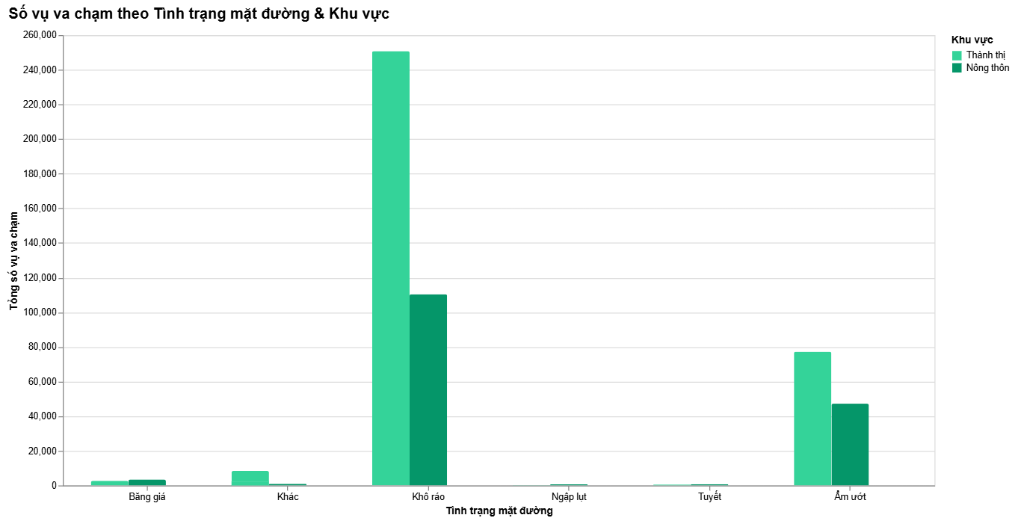
\includegraphics[width=\textwidth, keepaspectratio]{images/memberB_surface_area.png}
        \caption{Mặt đường và Khu vực}
    \end{subfigure}
    \hfill
    \begin{subfigure}{0.48\textwidth}
        \centering
        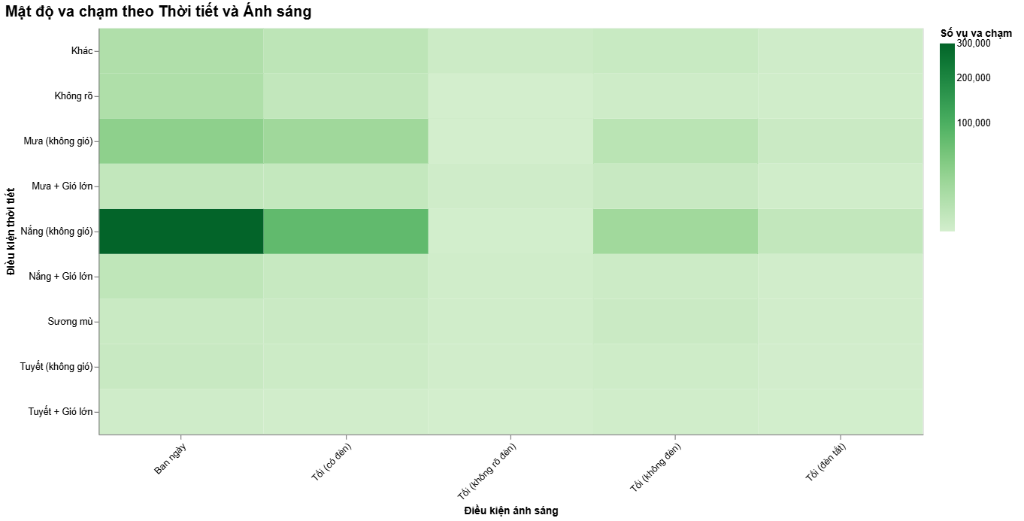
\includegraphics[width=\textwidth, keepaspectratio]{images/memberB_weather_light.png}
        \caption{Thời tiết và Ánh sáng}
    \end{subfigure}

    \vspace{0.3cm}

    \begin{subfigure}{0.48\textwidth}
        \centering
        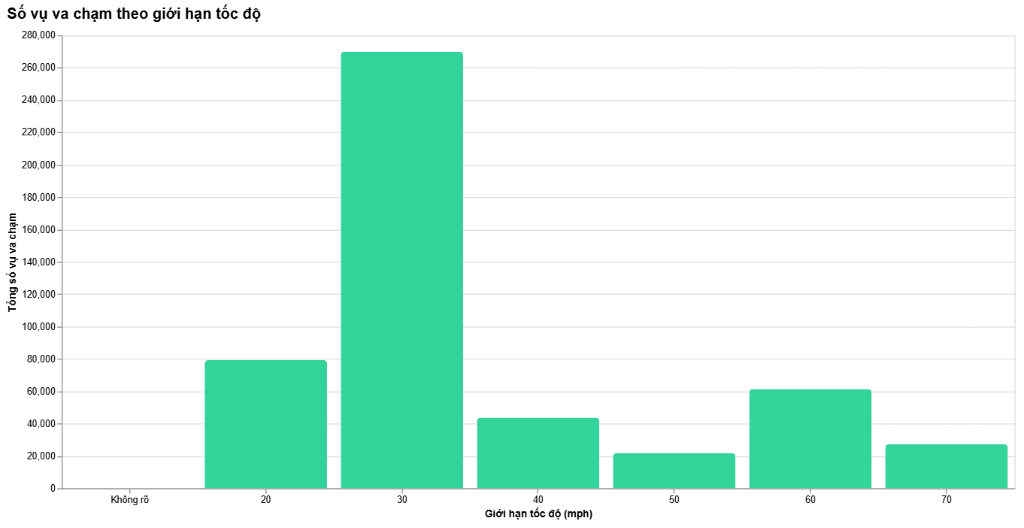
\includegraphics[width=\textwidth, keepaspectratio]{images/memberB_speed_limit.png}
        \caption{Va chạm theo giới hạn tốc độ}
    \end{subfigure}
    \hfill
    \begin{subfigure}{0.48\textwidth}
        \centering
        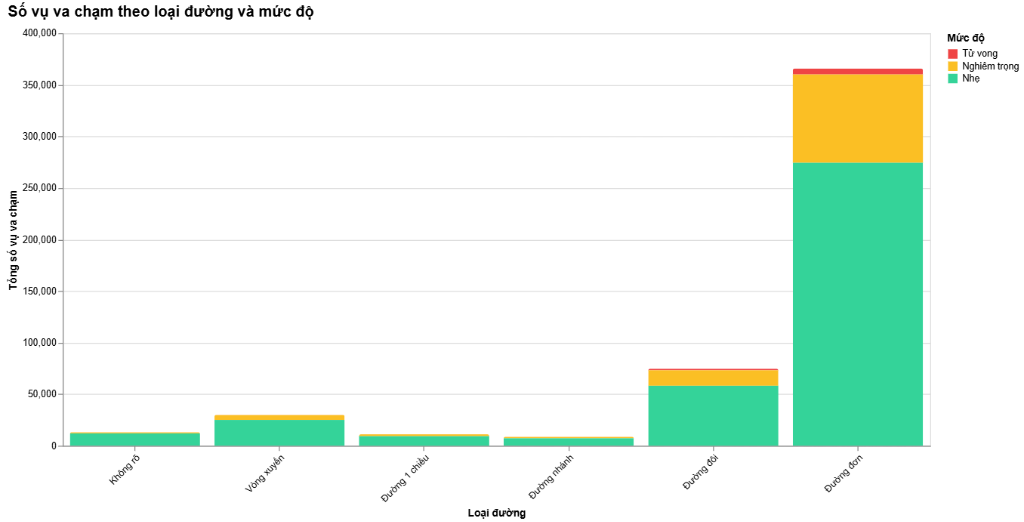
\includegraphics[width=\textwidth, keepaspectratio]{images/memberB_road_type.png}
        \caption{Loại đường và mức độ}
    \end{subfigure}
    \caption{Các biểu đồ phân tích Điều kiện đường sá và môi trường}
    \label{fig:memberB_charts}
\end{figure}

\subsection{Phương tiện và người lái}

\textbf{Mục tiêu}: Phân tích đặc điểm phương tiện và người lái trong các vụ va chạm, từ đó nhận diện nhóm phương tiện hoặc nhóm người lái xuất hiện nhiều trong các vụ tai nạn nghiêm trọng.

\textbf{Biểu đồ thực tế}:
\begin{itemize}
    \item Biểu đồ cột ngang (Bar chart): Thể hiện Top 10 loại phương tiện xuất hiện nhiều nhất trong các vụ va chạm.
    \item Biểu đồ vòng (Donut chart): Thể hiện tỷ lệ phương tiện tham gia va chạm theo khu vực Thành thị/Nông thôn.
    \item Biểu đồ cột xếp chồng (Stacked Column Chart): So sánh số phương tiện theo nhóm tuổi và giới tính người lái.
    \item Biểu đồ kết hợp cột và đường (Combo Chart): Đối chiếu số lượng phương tiện với số ca thương vong nặng theo nhóm tuổi.
\end{itemize}

\textbf{Nhận xét rút ra từ dữ liệu}:
\begin{itemize}
    \item \textbf{Ô tô chiếm ưu thế rất rõ}: Trong Top 10 loại phương tiện, nhóm Car vượt xa toàn bộ các nhóm còn lại. Các nhóm đứng sau như xe đạp, xe tải nhẹ và xe máy có số lượng thấp hơn nhiều, vì vậy khi đọc biểu đồ cần xem ô tô như nhóm nền chính của bức tranh va chạm.
    \item \textbf{Va chạm tập trung nhiều hơn ở Thành thị}: Biểu đồ vòng cho thấy khu vực Thành thị chiếm khoảng hai phần ba tổng số phương tiện liên quan đến va chạm, trong khi Nông thôn chiếm khoảng một phần ba. Chênh lệch này khá dễ hiểu nếu nhìn từ mật độ phương tiện và tần suất di chuyển trong khu vực đô thị.
    \item \textbf{Nhóm 26--35 tuổi nổi bật nhất}: Ở biểu đồ tuổi và giới tính, nhóm 26--35 có số phương tiện cao nhất, sau đó giảm dần qua các nhóm 36--45 và 46--55. Đây là nhóm tuổi tham gia giao thông thường xuyên, nên biểu đồ cho thấy họ xuất hiện nhiều trong các vụ va chạm hơn các nhóm quá trẻ hoặc cao tuổi.
    \item \textbf{Nam giới luôn cao hơn nữ giới ở hầu hết nhóm tuổi}: Các cột màu xanh của nam giới cao hơn rõ so với cột màu hồng ở gần như toàn bộ các nhóm tuổi. Đường thương vong nặng trong biểu đồ kết hợp cũng đạt đỉnh ở nhóm 26--35, rồi giảm dần ở các nhóm tuổi lớn hơn, khá tương đồng với xu hướng số phương tiện.
\end{itemize}

\begin{figure}[H]
    \centering
    \begin{subfigure}{0.48\textwidth}
        \centering
        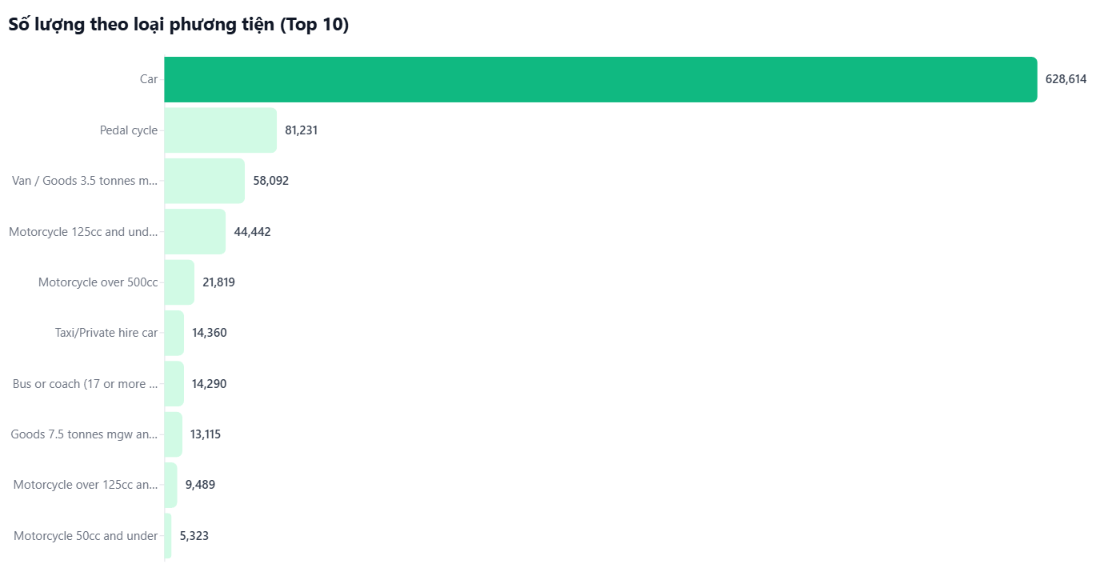
\includegraphics[width=\textwidth, keepaspectratio]{images/memberC_vehicle_type_top10.png}
        \caption{Top 10 loại phương tiện}
    \end{subfigure}
    \hfill
    \begin{subfigure}{0.48\textwidth}
        \centering
        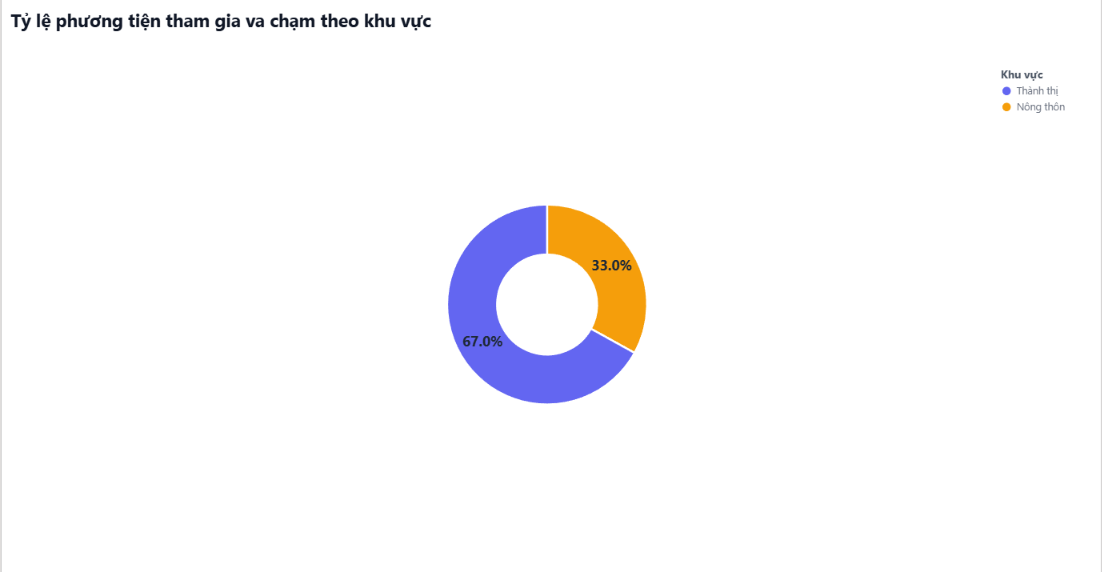
\includegraphics[width=\textwidth, keepaspectratio]{images/memberC_urban_rural_ratio.png}
        \caption{Tỷ lệ phương tiện theo khu vực}
    \end{subfigure}

    \vspace{0.3cm}

    \begin{subfigure}{0.48\textwidth}
        \centering
        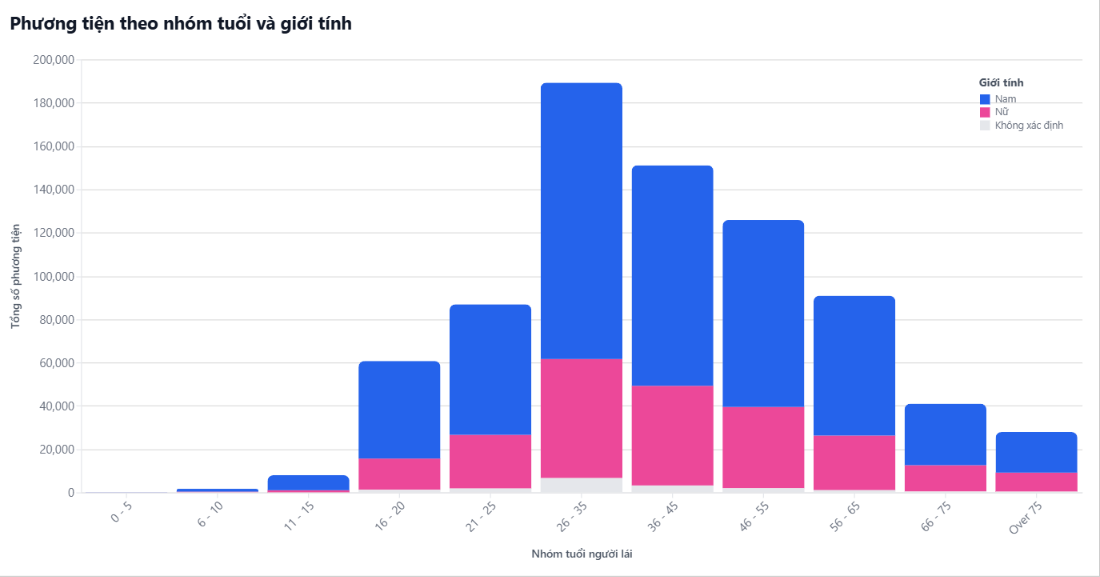
\includegraphics[width=\textwidth, keepaspectratio]{images/memberC_driver_age_gender.png}
        \caption{Nhóm tuổi và giới tính người lái}
    \end{subfigure}
    \hfill
    \begin{subfigure}{0.48\textwidth}
        \centering
        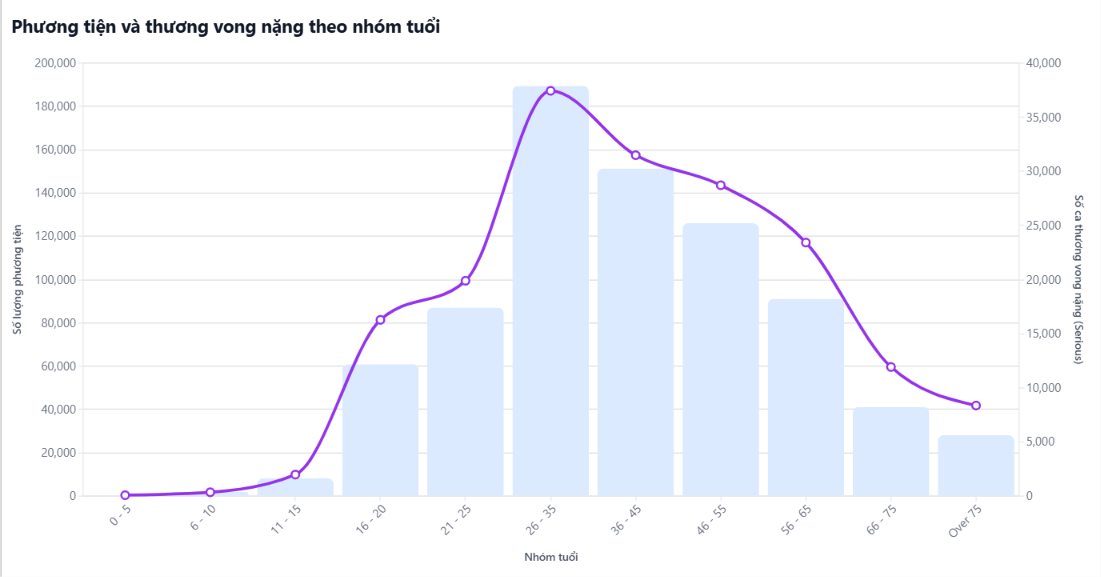
\includegraphics[width=\textwidth, keepaspectratio]{images/memberC_age_severe_casualties.png}
        \caption{Phương tiện và thương vong nặng theo tuổi}
    \end{subfigure}
    \caption{Các biểu đồ phân tích Phương tiện và người lái}
    \label{fig:memberC_charts}
\end{figure}

\subsection{Người thương vong và nhóm rủi ro}

\textbf{Mục tiêu}: Phân tích đặc điểm người thương vong theo độ tuổi, giới tính, vai trò tham gia giao thông và mức độ thương vong để xác định các nhóm rủi ro cao.

\textbf{Biểu đồ thực tế}:
\begin{itemize}
    \item Biểu đồ cột ngang (Bar chart): So sánh số người thương vong theo vai trò tham gia giao thông.
    \item Biểu đồ cột xếp chồng (Stacked Bar Chart): Thể hiện số người thương vong theo nhóm tuổi và mức độ nghiêm trọng.
    \item Biểu đồ cột nhóm (Clustered Column Chart): So sánh số người thương vong theo nhóm tuổi và giới tính.
    \item Biểu đồ cột 100\% xếp chồng (100\% Stacked Column Chart): So sánh tỷ lệ mức độ thương vong theo vai trò tham gia giao thông.
\end{itemize}

\textbf{Nhận xét rút ra từ dữ liệu}:
\begin{itemize}
    \item \textbf{Người điều khiển phương tiện chiếm nhiều nhất về số lượng}: Biểu đồ theo vai trò cho thấy nhóm Người điều khiển có số người thương vong lớn hơn hẳn Hành khách và Người đi bộ. Đây là nhóm trực tiếp tham gia điều khiển phương tiện, nên cũng là nhóm xuất hiện dày nhất trong thống kê thương vong.
    \item \textbf{Nhóm tuổi 26--35 là nhóm nổi bật nhất}: Khi phân theo tuổi và mức độ, nhóm 26--35 có tổng số thương vong cao nhất. Các nhóm 36--45 và 46--55 cũng còn ở mức cao, trong khi trẻ em và nhóm trên 66 tuổi thấp hơn rõ rệt về số lượng tuyệt đối.
    \item \textbf{Thương vong nhẹ vẫn chiếm phần lớn}: Ở hầu hết nhóm tuổi, phần màu xanh của mức độ Nhẹ là phần dài nhất trên thanh. Tuy vậy, phần Nghiêm trọng và Tử vong vẫn xuất hiện đều ở các nhóm tuổi trưởng thành, nên không thể chỉ nhìn tổng số cao mà bỏ qua mức độ hậu quả.
    \item \textbf{Người đi bộ có tỷ lệ hậu quả nặng đáng chú ý}: Nếu xét theo tỷ lệ, Người đi bộ có phần Nghiêm trọng và Tử vong lớn hơn hai nhóm còn lại. Nói cách khác, Người điều khiển là nhóm đông nhất về số lượng thương vong, nhưng Người đi bộ lại là nhóm cần chú ý nhiều hơn khi đánh giá mức độ nghiêm trọng.
    \item \textbf{Nam giới cao hơn nữ giới ở hầu hết nhóm tuổi}: Biểu đồ giới tính cho thấy cột Nam luôn cao hơn cột Nữ, đặc biệt rõ ở các nhóm tuổi 26--35, 36--45 và 46--55. Ở các nhóm tuổi cao hơn, khoảng cách này thu hẹp lại nhưng vẫn giữ cùng chiều hướng.
\end{itemize}

\begin{figure}[H]
    \centering
    \begin{subfigure}{0.48\textwidth}
        \centering
        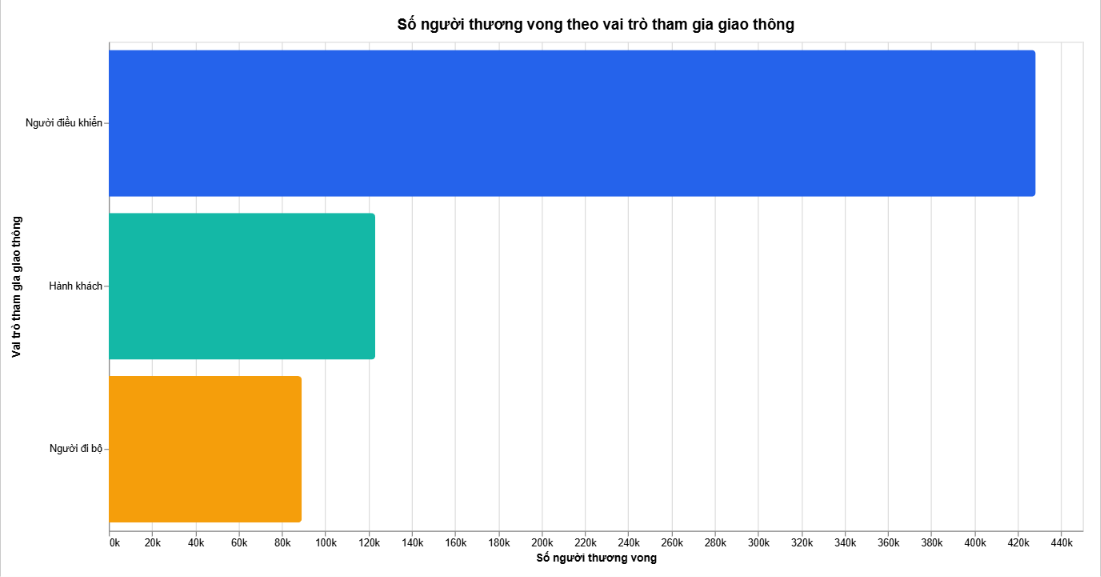
\includegraphics[width=\textwidth, keepaspectratio]{images/memberD_casualties_by_role.png}
        \caption{Thương vong theo vai trò}
    \end{subfigure}
    \hfill
    \begin{subfigure}{0.48\textwidth}
        \centering
        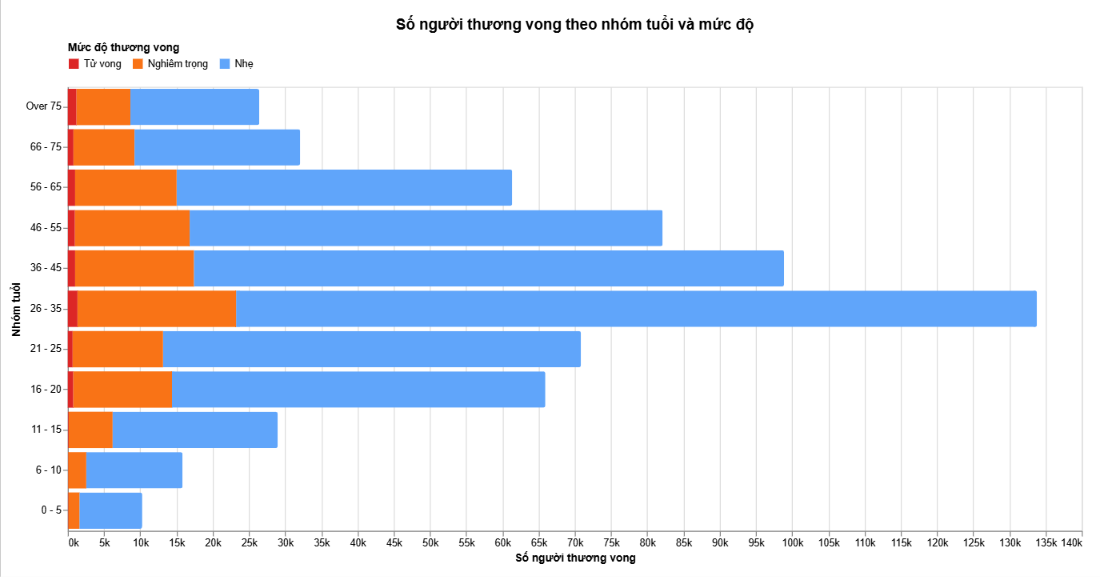
\includegraphics[width=\textwidth, keepaspectratio]{images/memberD_age_severity.png}
        \caption{Nhóm tuổi và mức độ thương vong}
    \end{subfigure}

    \vspace{0.3cm}

    \begin{subfigure}{0.48\textwidth}
        \centering
        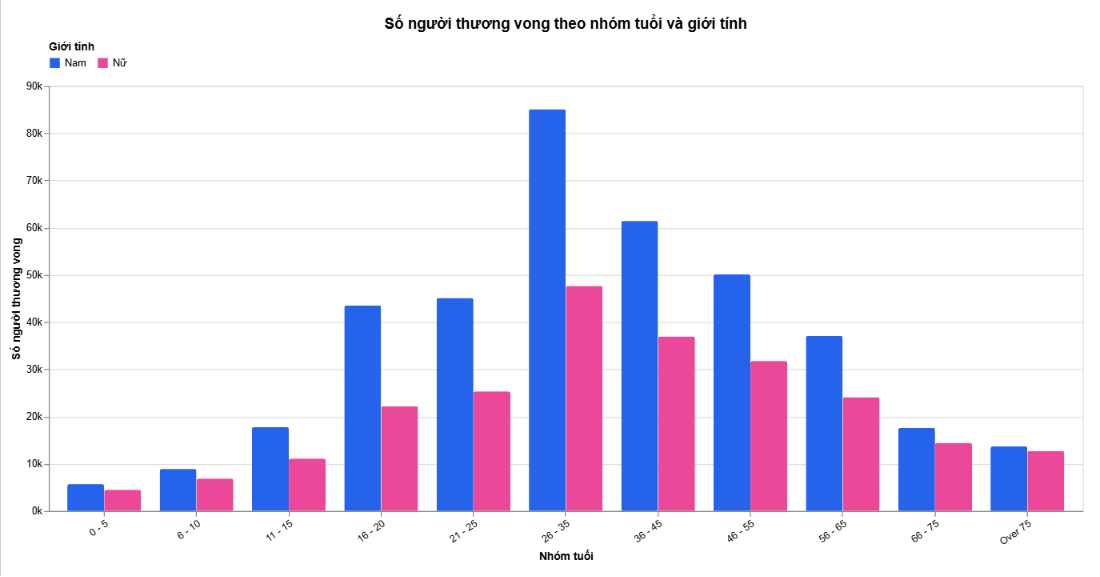
\includegraphics[width=\textwidth, keepaspectratio]{images/memberD_age_gender.png}
        \caption{Nhóm tuổi và giới tính}
    \end{subfigure}
    \hfill
    \begin{subfigure}{0.48\textwidth}
        \centering
        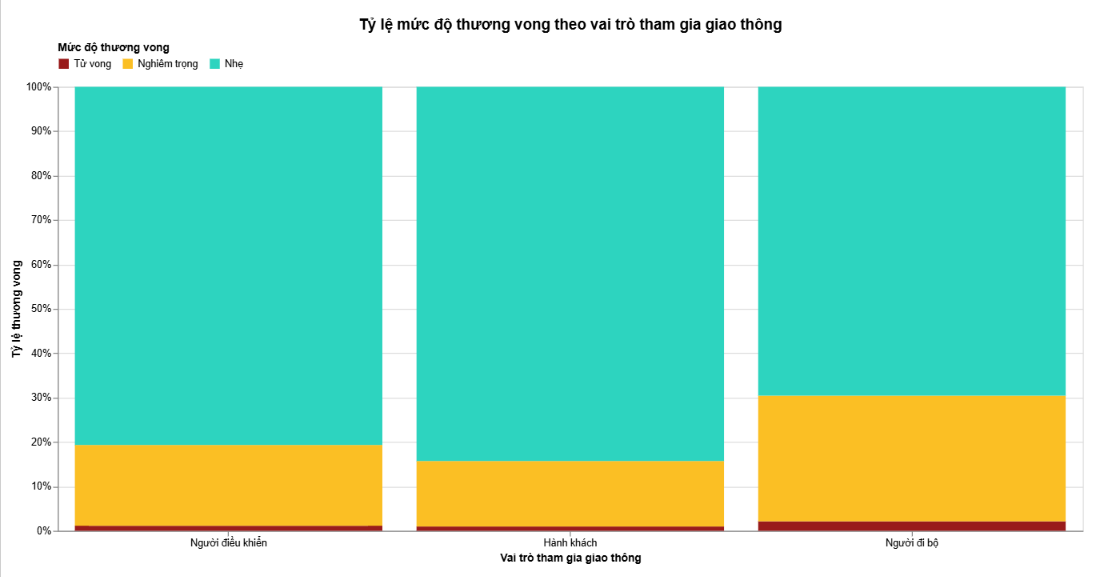
\includegraphics[width=\textwidth, keepaspectratio]{images/memberD_role_severity_ratio.png}
        \caption{Tỷ lệ mức độ theo vai trò}
    \end{subfigure}
    \caption{Các biểu đồ phân tích Người thương vong và nhóm rủi ro}
    \label{fig:memberD_charts}
\end{figure}

\subsection{Giao diện dashboard tổng hợp}

Sau khi hoàn thành các biểu đồ thành phần, nhóm đã tổng hợp và xây dựng một hệ thống dashboard tương tác gồm 5 trang báo cáo chuyên sâu trong Power BI. Hệ thống dashboard được thiết kế nhất quán với thanh điều hướng (navigation bar) ở bên trái, hàng thẻ KPI tổng hợp ở trên cùng, các bộ lọc (slicers) Dropdown ở góc trên bên phải và lưới biểu đồ chi tiết ở trung tâm.

Dưới đây là chi tiết giao diện thực tế của 5 trang báo cáo đã được hoàn thiện:

\begin{figure}[H]
    \centering
    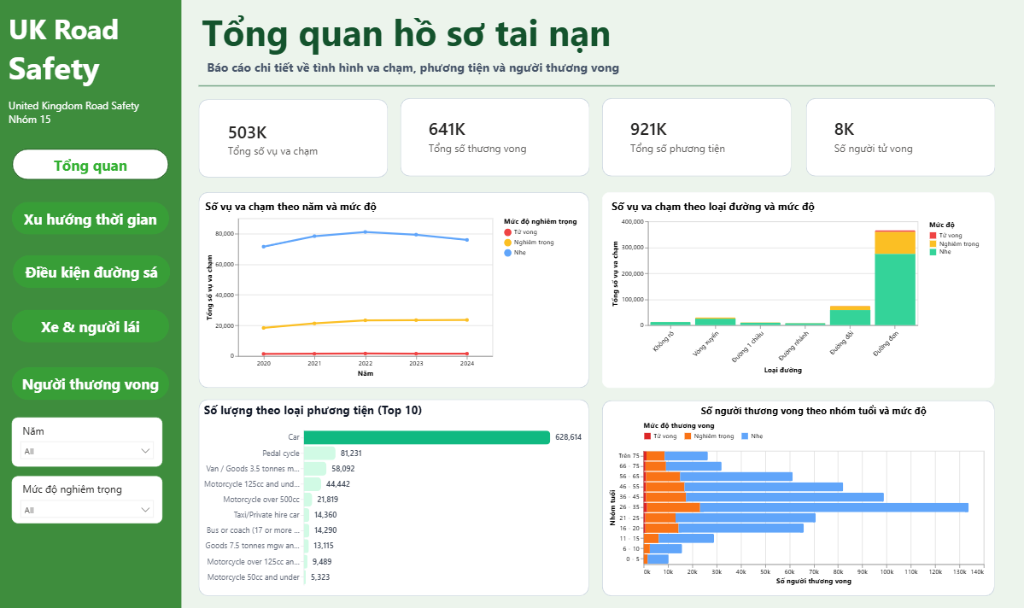
\includegraphics[width=0.75\textwidth, keepaspectratio]{images/dashboard_page1.png}
    \caption{Tổng quan hồ sơ tai nạn}
    \label{fig:dashboard_page1}
\end{figure}

\textbf{Tổng quan hồ sơ tai nạn} (Hình~\ref{fig:dashboard_page1}) cung cấp cái nhìn toàn cảnh về quy mô dữ liệu với 4 thẻ KPI chính: tổng số vụ va chạm (503K), tổng số thương vong (641K), tổng số phương tiện liên quan (921K) và số người tử vong (8K). Đồng thời tích hợp các biểu đồ quan trọng nhất từ các mục tiêu để người quản trị có góc nhìn bao quát tức thì.

\begin{figure}[H]
    \centering
    \begin{subfigure}[t]{0.48\textwidth}
        \centering
        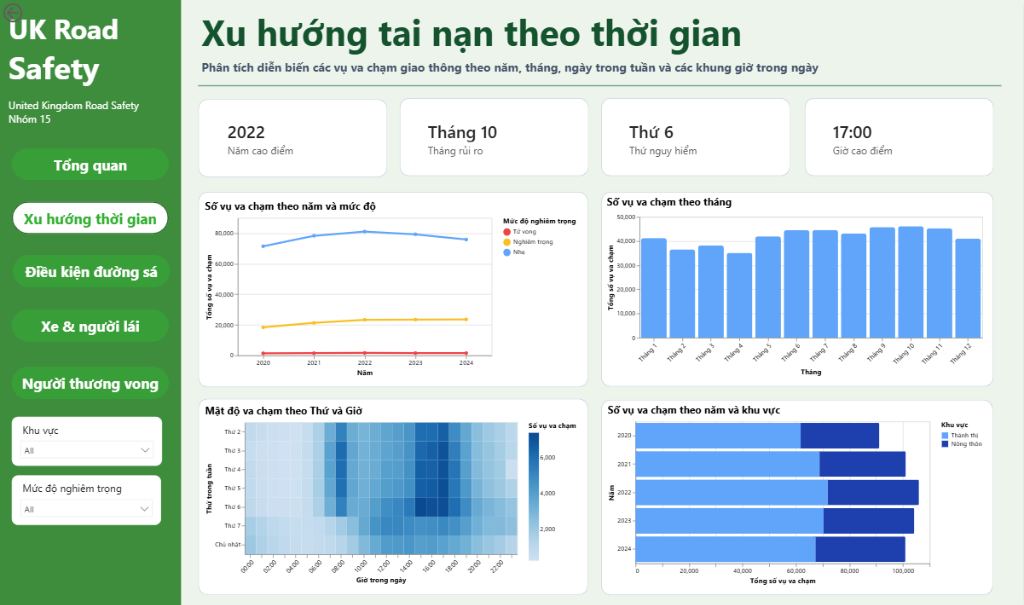
\includegraphics[width=\textwidth, keepaspectratio]{images/dashboard_page2.png}
        \caption{Xu hướng thời gian}
        \label{fig:dashboard_page2}
    \end{subfigure}
    \hfill
    \begin{subfigure}[t]{0.48\textwidth}
        \centering
        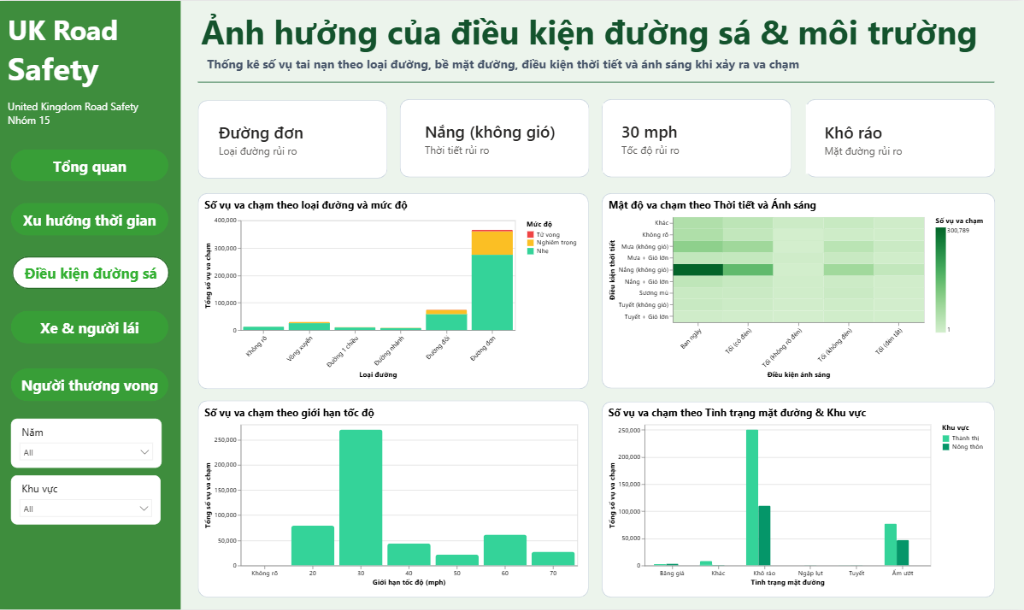
\includegraphics[width=\textwidth, keepaspectratio]{images/dashboard_page3.png}
        \caption{Điều kiện đường sá và môi trường}
        \label{fig:dashboard_page3}
    \end{subfigure}
    \caption{Giao diện trang Xu hướng thời gian và Điều kiện đường sá}
    \label{fig:dashboard_group1}
\end{figure}

\textbf{Phân tích xu hướng tai nạn theo thời gian} (Hình~\ref{fig:dashboard_page2}) tập trung vào làm rõ các mốc thời gian xảy ra tai nạn. Các thẻ KPI làm nổi bật các đỉnh điểm rủi ro: năm cao điểm (2022), tháng rủi ro (tháng 10), ngày nguy hiểm nhất trong tuần (thứ 6) và giờ cao điểm va chạm (17:00).

\textbf{Ảnh hưởng của điều kiện đường sá và môi trường} (Hình~\ref{fig:dashboard_page3}) phân tích các yếu tố hạ tầng và ngoại cảnh. Thẻ KPI thể hiện các điều kiện ghi nhận số tai nạn lớn nhất: loại đường đơn rủi ro nhất (Single carriageway), thời tiết nắng ấm (Fine no high winds), giới hạn tốc độ nội đô (30 mph) và tình trạng mặt đường khô ráo (Dry).

\begin{figure}[H]
    \centering
    \begin{subfigure}[t]{0.48\textwidth}
        \centering
        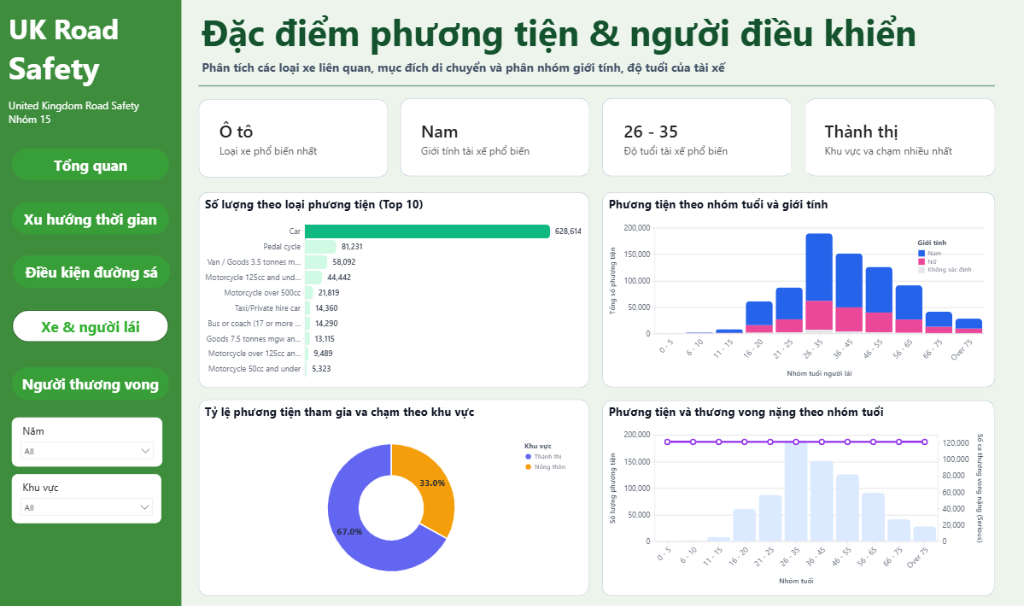
\includegraphics[width=\textwidth, keepaspectratio]{images/dashboard_page4.png}
        \caption{Phương tiện và người điều khiển}
        \label{fig:dashboard_page4}
    \end{subfigure}
    \hfill
    \begin{subfigure}[t]{0.48\textwidth}
        \centering
        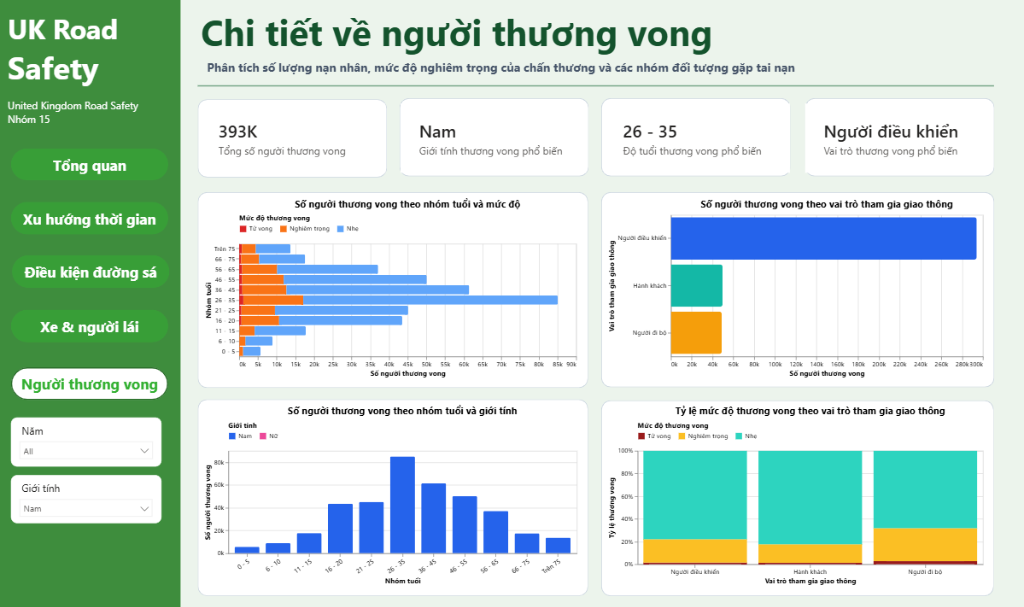
\includegraphics[width=\textwidth, keepaspectratio]{images/dashboard_page5.png}
        \caption{Người thương vong và nhóm rủi ro}
        \label{fig:dashboard_page5}
    \end{subfigure}
    \caption{Giao diện trang Phương tiện \& người điều khiển và Người thương vong}
    \label{fig:dashboard_group2}
\end{figure}

\textbf{Đặc điểm phương tiện và người điều khiển} (Hình~\ref{fig:dashboard_page4}) phân tích các khía cạnh liên quan tới phương tiện và tài xế. Thẻ KPI tổng hợp cho thấy loại phương tiện phổ biến nhất là Ô tô (Car), giới tính tài xế gặp nạn nhiều nhất là Nam, độ tuổi tài xế phổ biến nhất là từ 26--35 tuổi, và khu vực đô thị (Thành thị) chiếm tỷ trọng vượt trội (67%).

\textbf{Chi tiết về người thương vong và nhóm rủi ro} (Hình~\ref{fig:dashboard_page5}) tập trung sâu vào nạn nhân của các vụ tai nạn. Thẻ KPI thể hiện giới tính nạn nhân phổ biến là Nam, nhóm tuổi nạn nhân gặp rủi ro cao nhất là 26--35 tuổi, và vai trò của người thương vong phổ biến nhất là Người điều khiển phương tiện (Driver or rider). Cổng slicer cho phép lọc động theo giới tính và năm để phục vụ phân tích drill-down.

